\section{Jupyter Notebookの使い方}\label{sec: Jupyter Notebookの使い方}
Pythonを用いてデータ解析を行ううえでは,
対話的コンピューティング向けにPython標準のシェルを機能強化した
IPythonが有用である.
IPythonには
外部プログラムからIPythonの機能を利用するための機構が用意されている.
その機構を用いたIPythonのフロントエンドの一つがJupyter Notebookである.
本節ではJupyter Notebookを用いてPythonコードを編集・実行する方法を説明する.

なお,IPythonの機能を利用してPythonのコードを編集・実行するというのは
Jupyter Notebookにとって副次的な機能に過ぎない.
Jupyter Notebookの主たる機能は,
ノートブックとよばれる,
コードと出力を文章中に埋め込んだ文書を作成する機能である.
この機能の詳細については
参考文献\cite{rossant2015ipython}や
公式ドキュメント
(\url{https://jupyter-notebook.readthedocs.io/en/latest/notebook.html})
などを参照されたい.


\subsection{ユーザインタフェースの特徴}


\subsubsection{ユーザインタフェースの構成要素}
Jupyter Notebookのユーザインタフェースは
Notebook Dashboard,Notebook Editor,およびFile Editorからなる.

Notebook DashboardはJupyter Notebookの起動直後に表示されるページで,
簡単なファイルマネージャとしての機能をもち,
新しいノートブックを作成したり,
既存のノートブックを開いたりするために用いられる.
また,動作中の計算エンジンを強制停止させる機能も備えている.

Notebook Editorは
Notebook Dashboardからノートブックを開いた際に表示されるページで,
その名の通りノートブックを編集するためのインタフェースである.
viに代表されるモーダルエディタ(モードをもつエディタ)の一種であり,
後述の二つのモードをもつ.

File Editorは
Notebook Dashboardからノートブック以外を開いた際に表示されるページで,
ごくシンプルなテキストエディタである.


\subsubsection{Notebook Editorのモード}
Notebook Editorはモーダルエディタであり,
編集モードとコマンドモードという二つのモードをもっている.
メニューバーの右方に[\,\faPencil\,]マークが表示されていれば編集モード,
表示されていなければコマンドモードになっている.

編集モードは,
セルにテキストを入力するといった
セル内部に対する操作を行うためのモードである.
編集モードに切り替えるには,
セルの入力領域をクリックするか,もしくは[Enter]キーを押す.

コマンドモードは,
セルの新規作成などのセル単位での操作や
ノートブックの保存のようなノートブック全体に関する操作を
行うためのモードである.
コマンドモードに切り替えるには,
入力領域以外をクリックするか,もしくは[Esc]キーを押す.


\subsection{基本的な操作方法}


\subsubsection{Jupyter Notebookの起動}
コマンドプロンプト(cmd.exe)もしくはターミナルを開き,
作業用のディレクトリに移動したうえで
\verb|jupyter notebook|コマンドを実行する.


\subsubsection{ノートブックの新規作成}
Notebook Dashboardにおいて,
右上の[New]ボタンを押し,
表示されたリストの中から
使用する計算エンジン(「Python [Root]」または「Python 3」)を選択する
(図\ref{fig: ノートブックの新規作成})\footnote{%
ブラウザからローカルのプログラムが実行されることになるので,
一部のウイルス対策ソフトウェアは
このときPythonをウイルスと判定してしまう.
ウイルスと判定された場合,
(この問題であることを十分に確認したうえで)Pythonを例外に追加する.
}.

\begin{figure}[htbp]
\centering
\setlength{\fboxsep}{0pt}
\fcolorbox{gray}{gray}{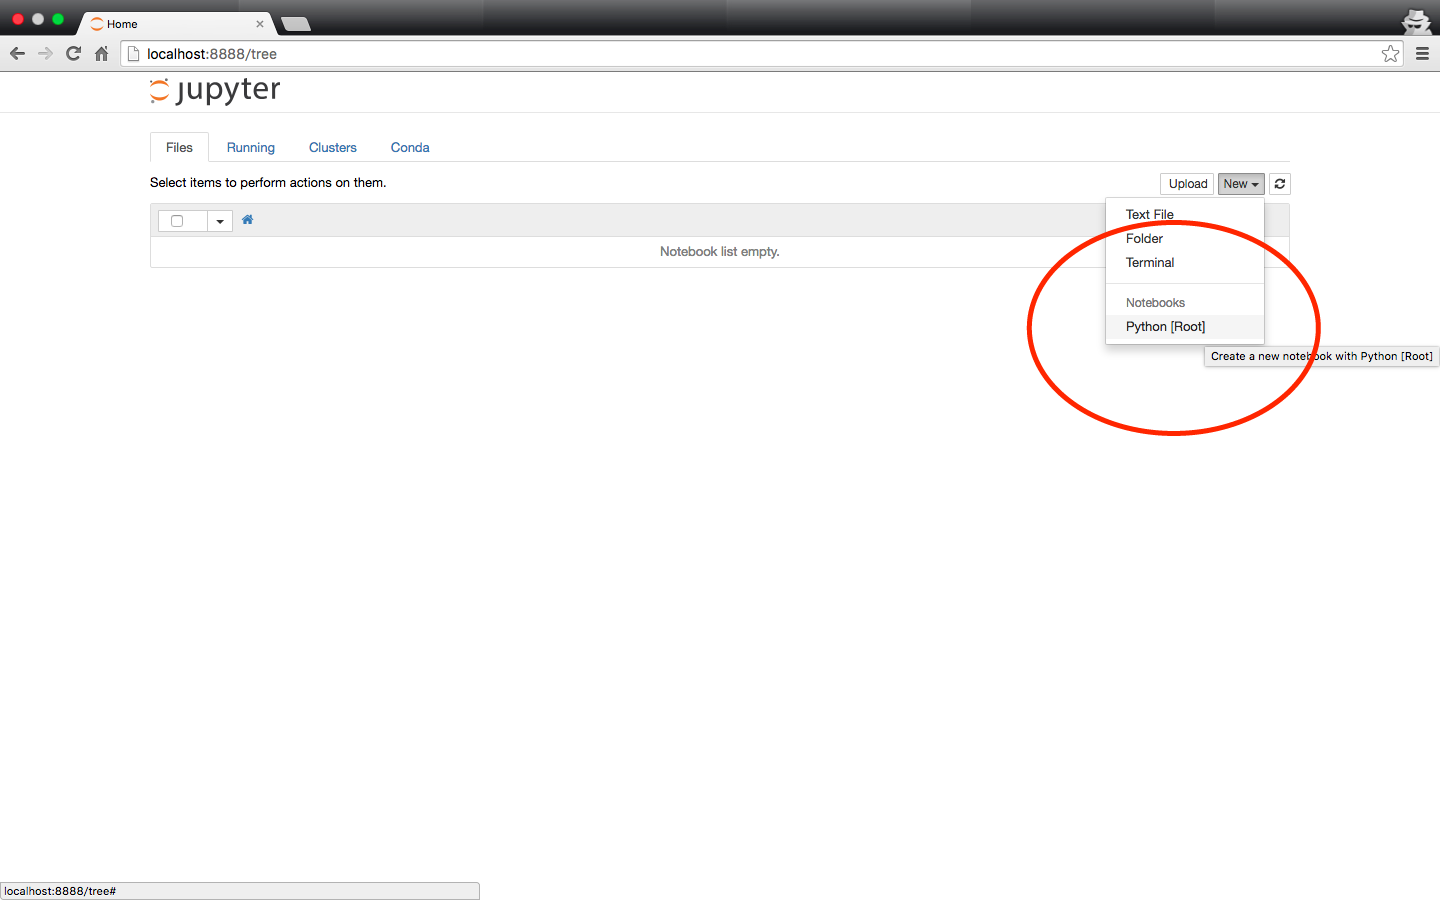
\includegraphics[scale=.25]{graphics/jupyter_10.png}}
\caption{\label{fig: ノートブックの新規作成}%
ノートブックの新規作成.
}
\end{figure}


\subsubsection{既存ノートブックの読み込み}
開きたいノートブック(拡張子ipynbのファイル)
をNotebook Dashboardから選択する.


\subsubsection{Pythonコードの入力}
Notebook Editorにおいて以下のように操作する.
\begin{enumerate}
\item
コードを入力したいセルを選択する.
\item
ツールバーのプルダウンメニューにおいて
セルタイプ「Code」が選択されていることを確認する.
セルタイプが「Code」以外になっている場合は,
プルダウンメニューからセルタイプ「Code」を選択するか,
コマンドモードに切り替えてキーボードショートカット[y]を使用する.
\item
編集モードに切り替え,セルにコードを入力する
(図\ref{fig: Pythonコードの入力}).

\begin{figure}[htbp]
\centering
\setlength{\fboxsep}{0pt}
\fcolorbox{gray}{gray}{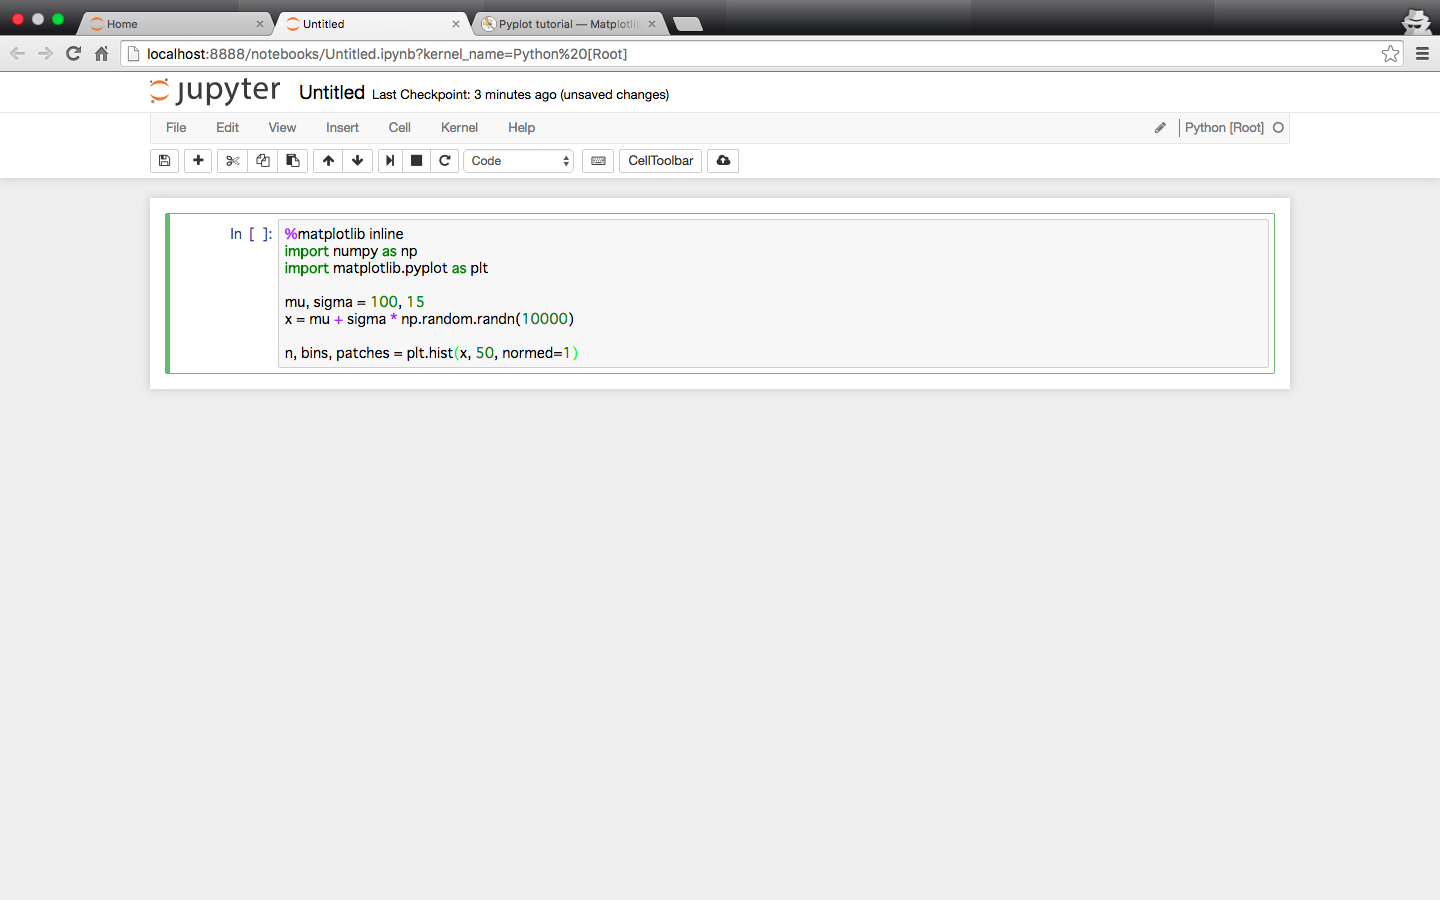
\includegraphics[scale=.25]{graphics/jupyter_06.png}}
\caption{\label{fig: Pythonコードの入力}%
Pythonコードの入力.
}
\end{figure}
\end{enumerate}


\subsubsection{Pythonコードの実行}
Notebook Editorにおいて以下のように操作する.
\begin{enumerate}
\item
実行したいコードが入力されたセルを選択する.
\item
ツールバーの[\,\faStepForward\,]ボタンを押すか,
キーボードショートカット[Shift]+[Enter]
(コマンドモード/編集モードのいずれでも使用可)
を使用する.
実行中のセルはセル番号が\verb|In [*]|と表示される.
\end{enumerate}


\subsubsection{ノートブック名の変更}
Notebook Editorの上部,Jupyterロゴの横に表示されている
ノートブック名をクリックし,
新しいノートブック名を入力する
(図\ref{fig: ノートブック名の変更}).

\begin{figure}[htbp]
\centering
\setlength{\fboxsep}{0pt}
\fcolorbox{gray}{gray}{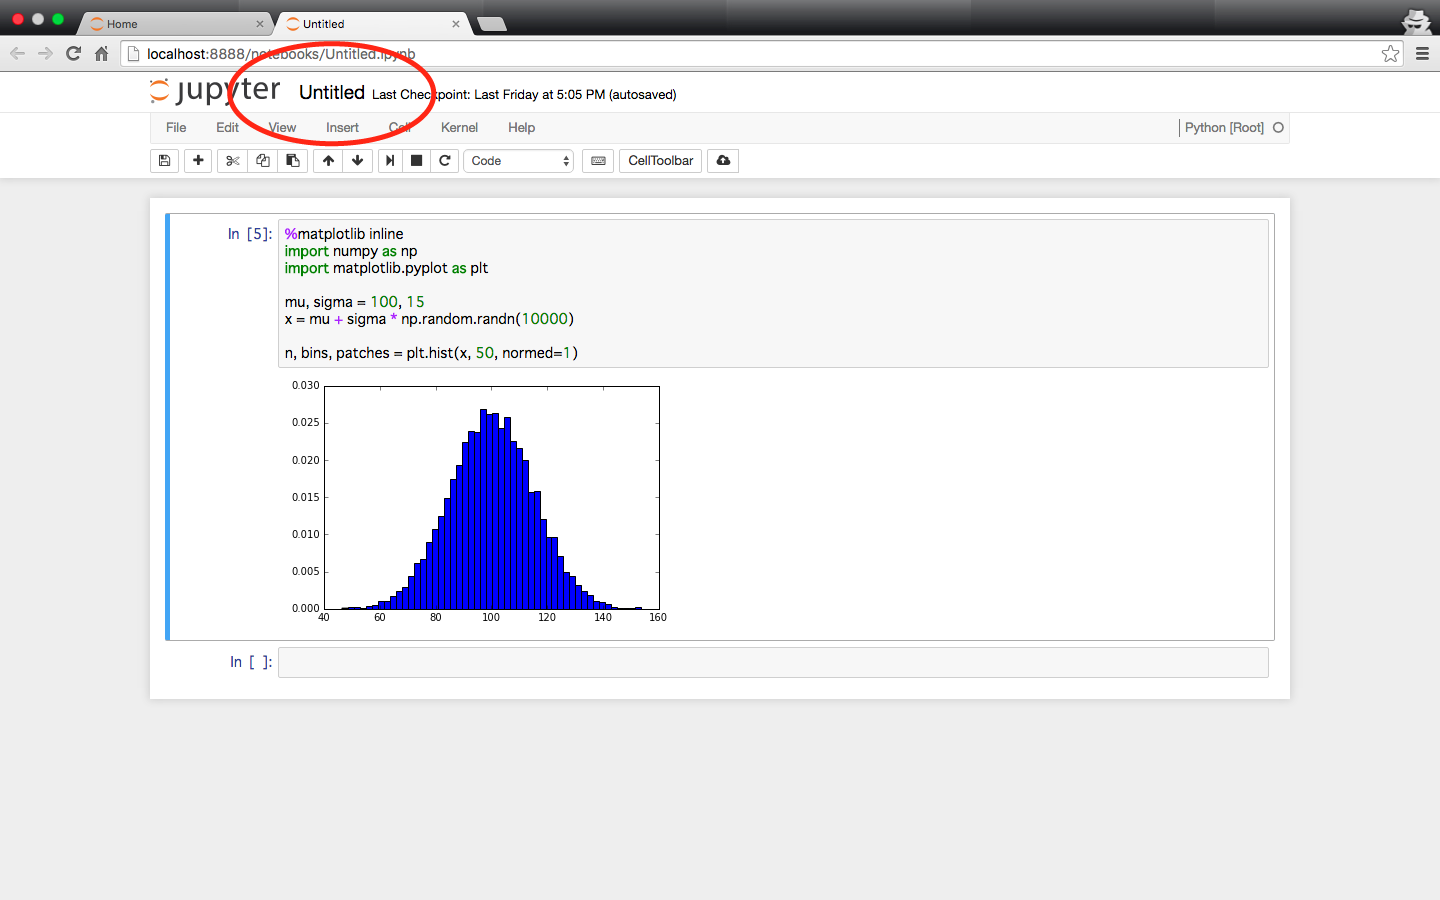
\includegraphics[scale=.25]{graphics/jupyter_12.png}}
\caption{\label{fig: ノートブック名の変更}%
ノートブック名の変更.
}
\end{figure}


\subsubsection{ノートブックの上書き保存}
Notebook Editorにおいて,
ツールバーの[\,\faFloppyO\,]ボタンを押すか,
コマンドモードに切り替えてキーボードショートカット[s]を使用する.


\subsubsection{ノートブックの別名保存}
Notebook Editorの[File]メニューから[Make a Copy...]を選択する.


\subsubsection{Jupyter Notebookの終了}
\begin{enumerate}
\item
Notebook Editorの[File]メニューから[Close and Halt]を選択することで,
Notebook Editorを閉じると同時に計算エンジンを停止させる\footnote{%
計算エンジンを停止させずにNotebook Editorを閉じてしまった場合は,
Notebook Dashboardの[Running]タブを開き,
当該ノートブックの[Shutdown]ボタンを押して停止させる.
}.
\item
Notebook Dashboardを閉じる.
(ブラウザを閉じればよい.)
\item
シェル(コマンドプロンプトもしくはターミナル)
上に残ったサーバジョブを[Ctrl]+[c]キーで停止させる.
\end{enumerate}


\begin{thebibliography}{9}
\bibitem{rossant2015ipython}
Cyrille Rossant(著), 菊池彰(訳)『IPythonデータサイエンスクックブック: 対話型コンピューティングと可視化のためのレシピ集』(オライリージャパン).
\end{thebibliography}
